\resizebox{7.5cm}{7.5cm}{
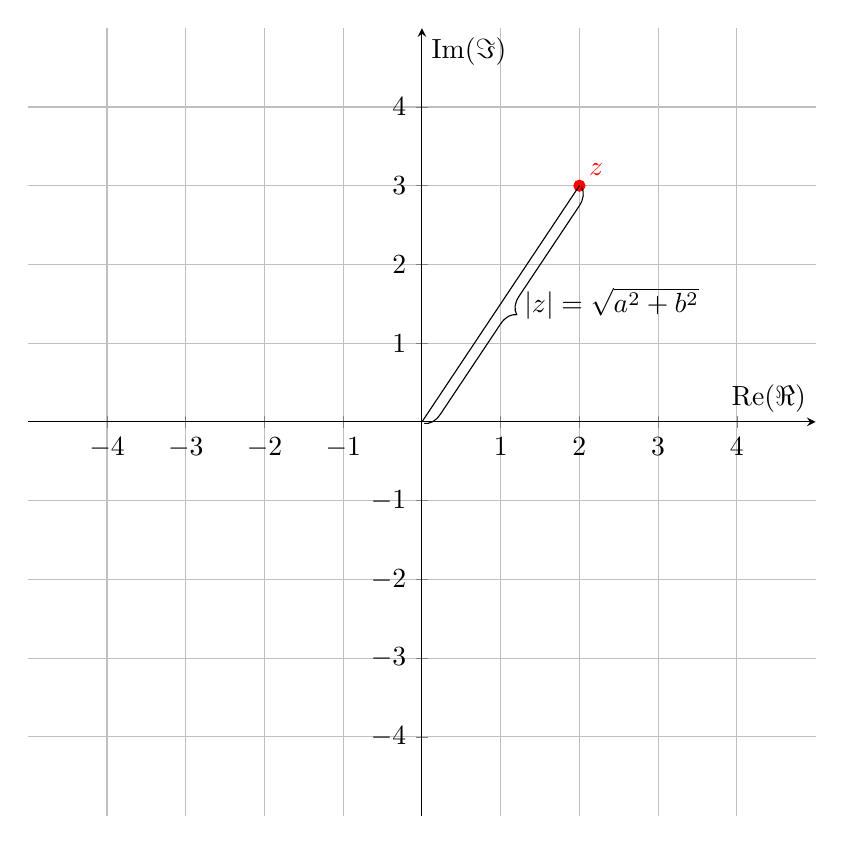
\begin{tikzpicture}
    \begin{axis}[
        samples=100,
        axis lines=center,
        x=1cm,
        y=1cm,
        xmin=-5, xmax=5,
        ymin=-5, ymax=5,
        xtick={-4, -3,...,3, 4},
        ytick={-4, -3,...,3, 4},
        xticklabels={$-4$,$-3$,$-2$,$-1$,$0$,$1$,$2$,$3$,$4$},
        yticklabels={$-4$,$-3$,$-2$,$-1$,$0$,$1$,$2$,$3$,$4$},
        xlabel=$\mbox{Re} (\Re)$,
        ylabel=$\mbox{Im} (\Im)$,
        grid=major,
    ]

    \draw[color = red, fill] (2, 3) circle[radius=2pt, fill] node[above right]{$z$};
    
    %\draw[decorate, decoration = {brace,amplitude=6pt,raise=1pt}] (0, 3) -- (2, 3) node[midway, above, yshift=5pt]{a};
    %\draw[decorate, decoration = {brace,amplitude=6pt,raise=1pt,mirror}] (2, 0) -- (2, 3) node[midway, right, xshift=5pt]{b};

    \draw[decorate, decoration = {brace,amplitude=6pt,raise=1pt,mirror}] (0, 0) -- (2, 3) node[midway, right, xshift=5pt]{$\left| z \right| = \sqrt{a^2 + b^2} $};
    \draw[] (0, 0) -- (2, 3);

    \end{axis}
\end{tikzpicture}
}
